\subsection{Cambios de vías}
    \label{sec:switches}
 	Un cambio de vías es un elemento ferroviario dinámico, que puede adoptar diferentes posiciones que modifican la topología de la red. Una formación por si sola no puede hacer mas que avanzar o retroceder, pero utilizando un cambio de vías es posible trazar nuevos caminos en el tendido ferroviario, modificando la posición de los cambios de vías.
 	
 	Los cambios de vías pueden ser simples, dobles o en tijeras. Las posiciones que pueden adoptar se visualizan en la Figura \ref{fig:cambios_0}. Un cambio de vías simple permite dos circulaciones posibles, una por vía principal y otra por vía secundaria. Un cambio de vías dobles permite cuatro circulaciones posibles, todas de igual prioridad. Un cambio de vías en tijeras permite dos circulaciones posibles, ambas principales.
 	
 	\begin{figure}[H]
 		\centering
 		\includegraphics[width=1\textwidth]{Figuras/circulacion.png}
 		\centering\caption{Circulaciones posibles en cambios de vías.}
 		\label{fig:cambios_0}
 	\end{figure}
 	
 	El sistema de enclavamientos modifica la posición de los cambios de vías por medio de una máquina de cambios. Una máquina de cambios (Figura \ref{fig:cambios_1}) es un mecanismo utilizado para permitir el paso de las formaciones de una vía a una ramificación del recorrido principal. Esto se realiza mediante el movimiento de la aguja del cambio (riel móvil) hacia su respectiva contraaguja (riel fijo) hasta obtener un adecuado acoplamiento que permita la circulación de la formación.

    \begin{figure}[H]
        \centering
        \includegraphics[width=0.75\textwidth]{Figuras/Cambios.jpg}
        \centering\caption{Máquina de cambios.}
        \label{fig:cambios_1}
    \end{figure}

    En la Figura \ref{fig:cambios_2} se muestra el cambio de vía de la estación Matheu de la Línea Mitre. Se observa que según sea la posición de la máquina de cambios, el tren puede continuar en la misma vía o hacer el cambio a la otra vía.

    \begin{figure}[H]
        \centering
        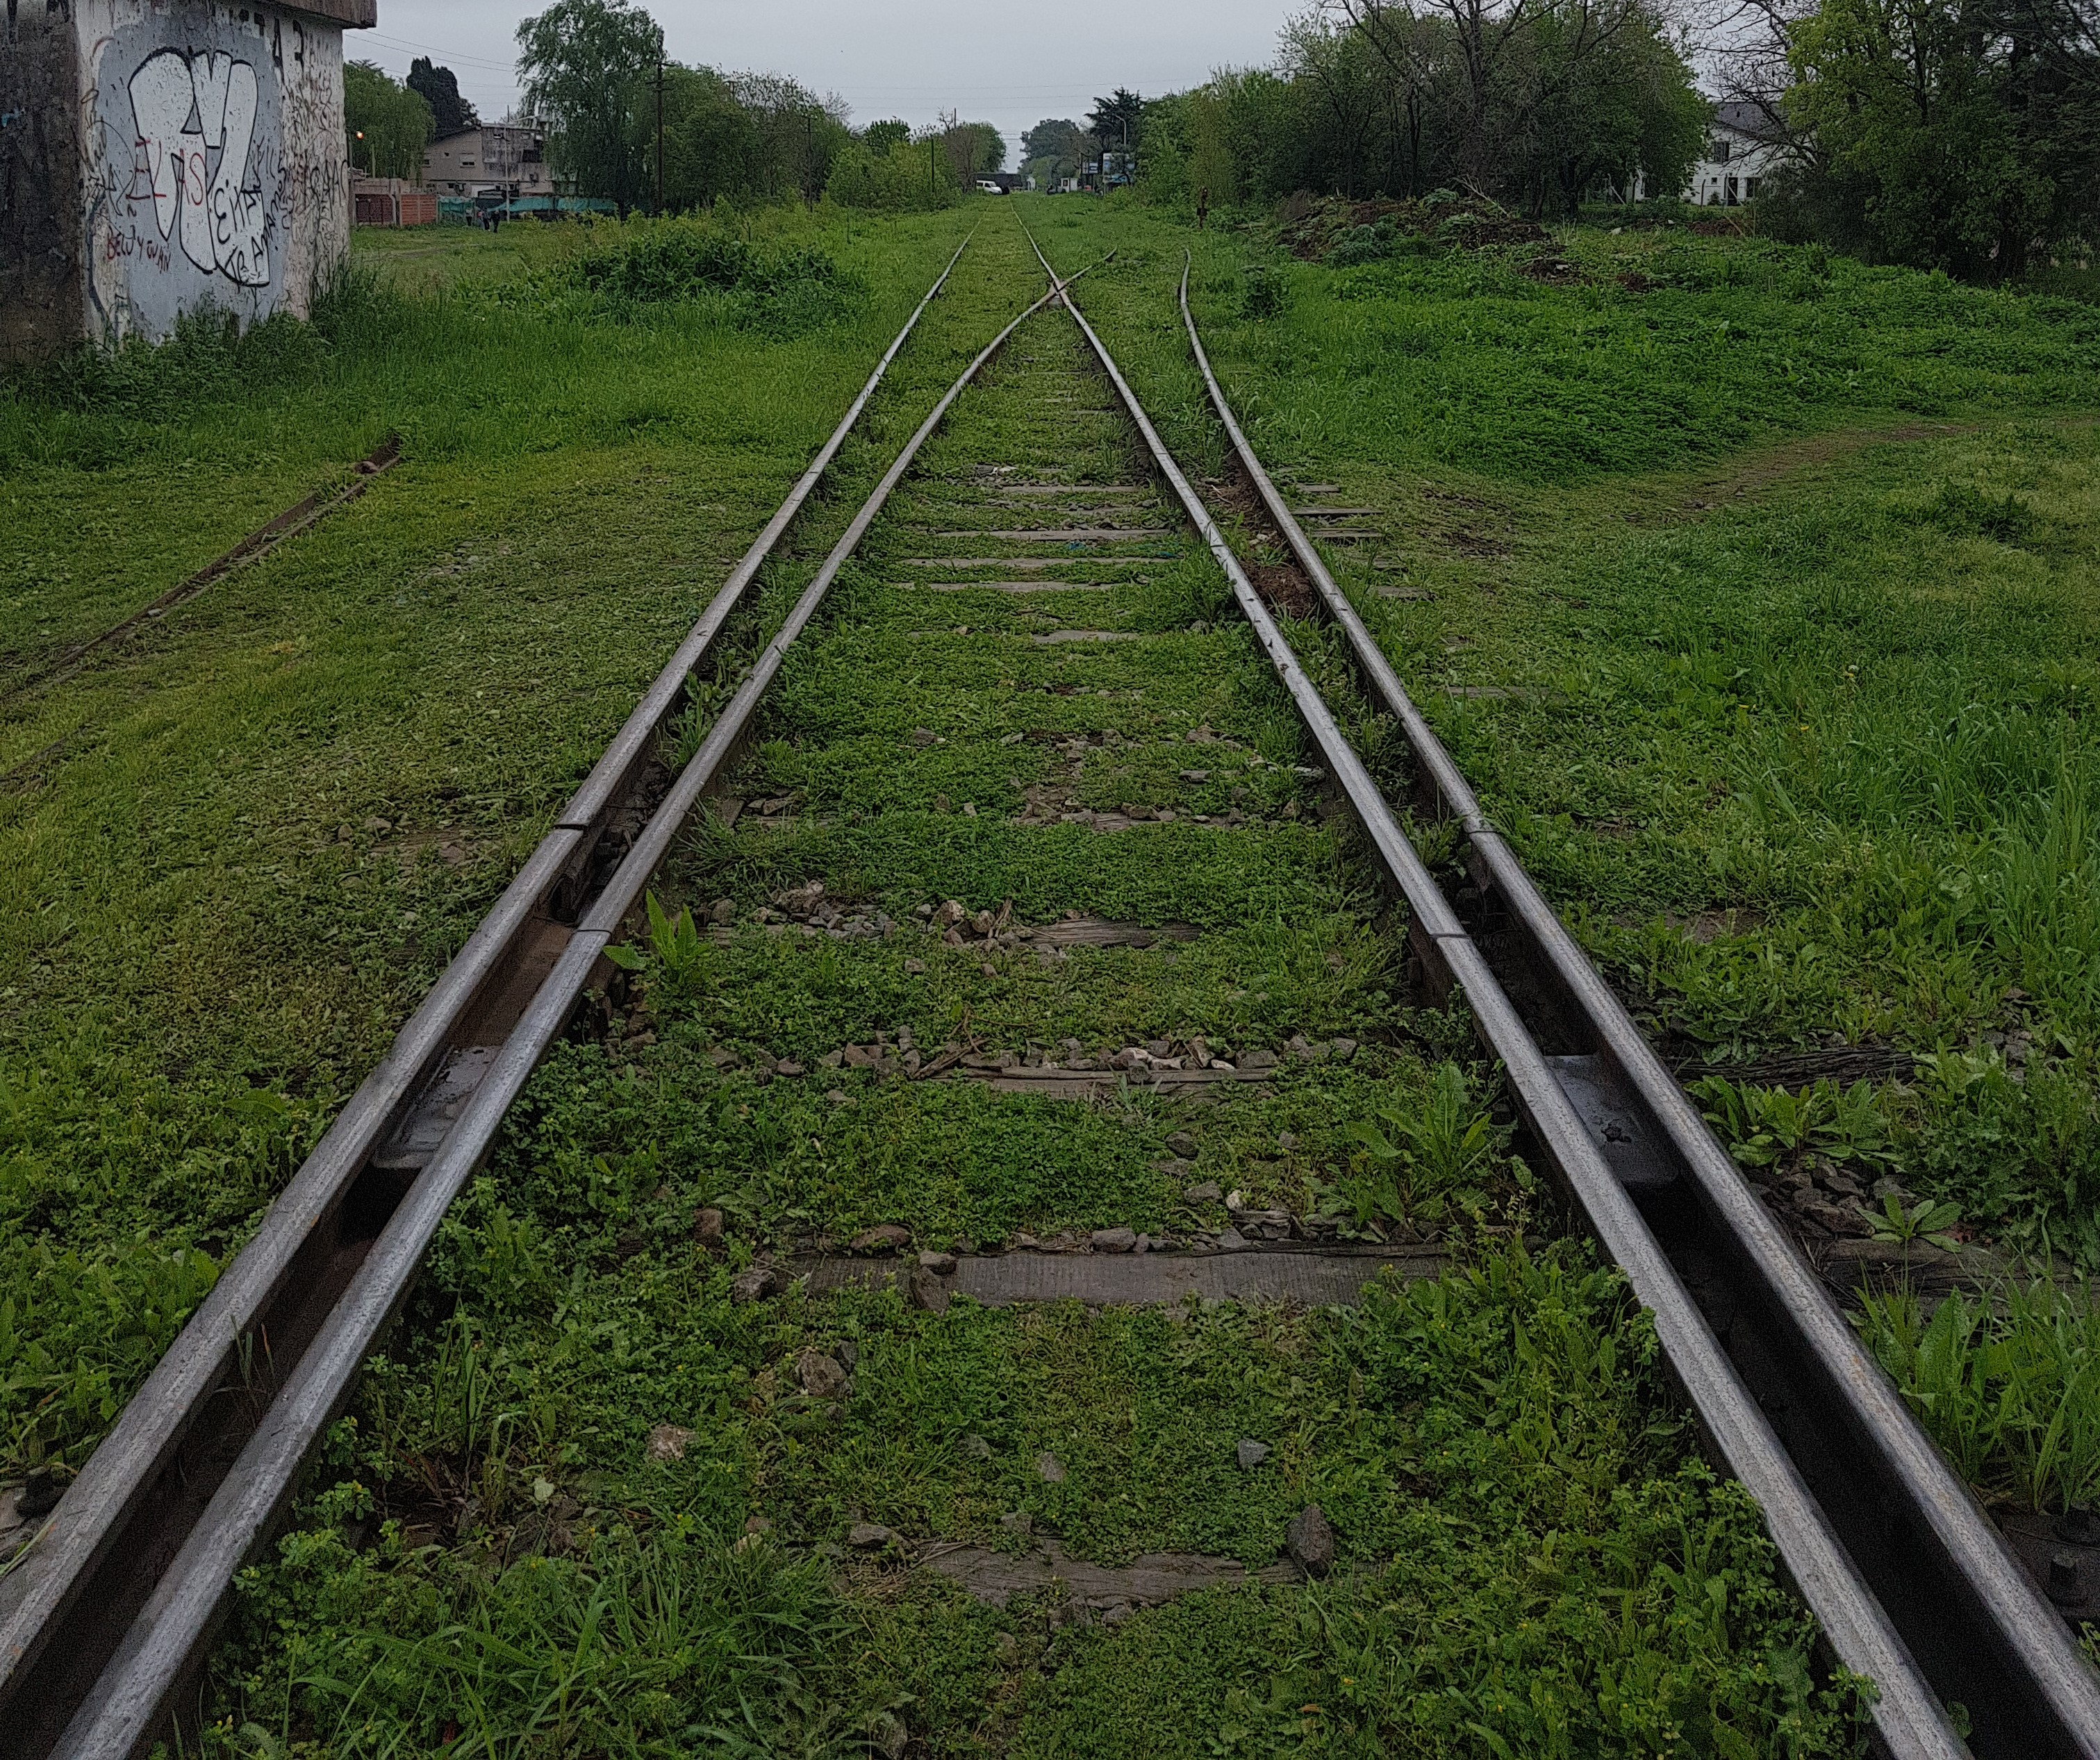
\includegraphics[width=0.75\textwidth]{Figuras/Cambios_2.jpg}
        \centering\caption{Cambio de vías de estación Matheu, Linea Mitre.}
        \label{fig:cambios_2}
    \end{figure}

    %En la Figura \ref{fig:cambios_3} se muestran las posiciones que puede adoptar el cambio. En la posición normal, los trenes pueden circular de forma directa, en paralelo, por la vía principal en sentidos opuestos. En la posición reversa, por el contrario, se permite el intercambio de trenes de una rama principal a otra en sentido opuesto o a una ramificación secundaria de la red.

   % \begin{figure}[H]
   %     \centering
   %     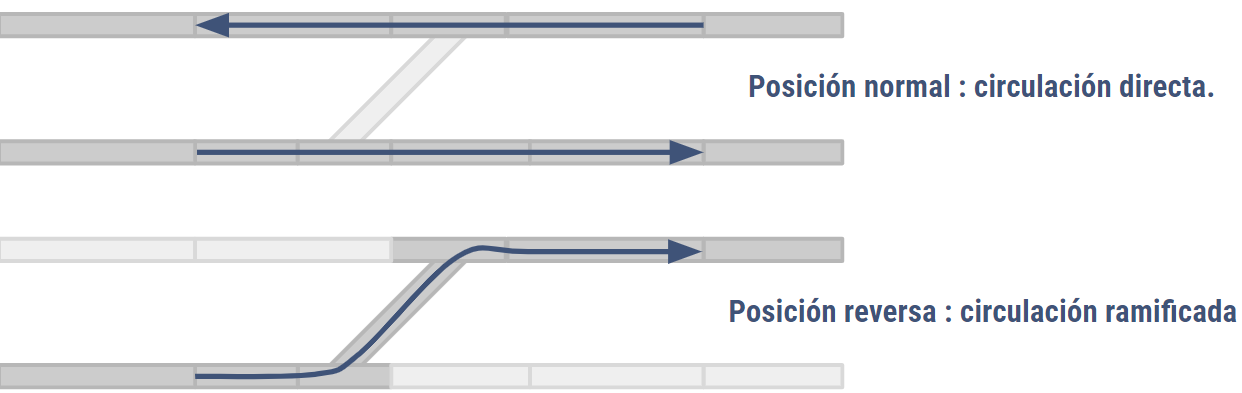
\includegraphics[width=1\textwidth]{Figuras/cambio_3.PNG}
   %     \centering\caption{Posiciones adoptadas por un cambio de vías simple.}
   %     \label{fig:cambios_3}
   % \end{figure}

    Al ser mecanismos que necesitan tiempo para cambiar de un estado al otro, no puede asumirse que el comando es obedecido al instante. Incluso podría darse el caso que jamás llegue a cumplirse la orden debido a desperfectos mecánicos o eléctricos. Es por eso que introducimos los conceptos de comando, indicación y correspondencia, tal como se ilustran en la Figura \ref{fig:cambios_4}.

    \begin{figure}[H]
        \centering
        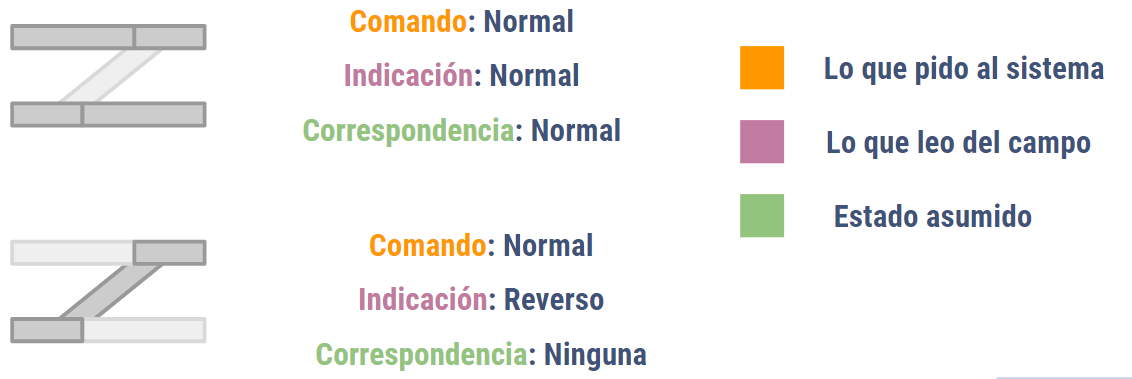
\includegraphics[width=1\textwidth]{Figuras/cambios}
   \textit{}     \centering\caption{Comando, indicación y correspondencia en un cambio de vías.}
        \label{fig:cambios_4}
    \end{figure}
    
    El comando es la instrucción que el sistema de enclavamientos envía a la máquina de cambios. Esta instrucción puede ser modificar la posición de normal a reverso o de reverso a normal. La indicación es el estado que la máquina de cambios informa al sistema de enclavamientos. El sistema solo asume que el comando fue obedecido cuando tanto el comando como la indicación muestran una correspondencia. En caso contrario, el sistema de enclavamiento no puede asumir cual es el estado real del sistema, si el comando enviado o el estado reportado por la máquina de cambios. El mismo concepto puede ser aplicado en cualquier otro elemento mecánico, como por ejemplo las barreras ferroviarias.

    El RNA debe analizar diversos atributos distribuidos entre la clase \textit{switchIS} (Código \ref{lst:switchIS}), la clase \textit{spotElementProjection} (Código \ref{lst:switch}) y la clase \textit{switchIL} (Código \ref{lst:switchIL}). La clase \textit{switchIS} se encuentra dentro del vector de clases \textit{switchesIS}, dentro de la clase \textit{functionalInfrastructure}, que a su vez es parte de la clase infrastructure. La clase \textit{switchIS} define el id de la máquina de cambios, el tipo (ordinario), el \textit{netElement} al cual pertenece la entrada del cambio y hacia que lado se encuentra la vía de continuación y ramificación si transitamos desde el \textit{netElement} del cambio hacia el cambio mismo. En este caso, si transitamos por el \textit{netElement} ne16 el tren tendrá la vía de continuación en la mano derecha y la ramificación en la mano izquierda. Los cambios de vías simples ("ordinarySwitch") siempre tienen una rama izquierda y una rama derecha definida. Además, dentro de la definición de cada rama tenemos el atributo \textit{netRelationRef}, del cual se puede obtener, procesamiento mediante, los otros \textit{netElement} correspondientes a las ramas: ne15 y ne14.

    \begin{lstlisting}[language = XML, caption = Clase \textit{switchIS} , label = {lst:switchIS}]
    <switchIS id="swi84" continueCourse="right" branchCourse="left" type="ordinarySwitch">
        <name name="Sw01" language="en"/>
        <spotLocation id="swi84_sloc01" netElementRef="ne16" applicationDirection="reverse" intrinsicCoord="0.0000"/>
        <designator register="_Example" entry="SWITCH Sw01"/>
        <leftBranch netRelationRef="nr_ne15ne16_swi84" branchingSpeed="0" joiningSpeed="0" radius="-500"/>
        <rightBranch netRelationRef="nr_ne14ne16_swi84" branchingSpeed="0" joiningSpeed="0" radius="0"/>
    </switchIS>
    \end{lstlisting}

    La clase \textit{spotElementProjection} define la ubicación en el espacio del elemento ferroviario referido. En este caso, como se puede ver en el Código \ref{lst:switch}, la posición de la máquina de cambios es la coordenada (-561 ; -450).

    \begin{lstlisting}[language = XML, caption = Clase \textit{spotElementProjection} , label = {lst:switch}]
    <spotElementProjection refersToElement="swi84" id="vis01_sep16">
        <name name="Sw01" language="en"/>
        <coordinate x="-560.994" y="-450.000"/>
    </spotElementProjection>
    \end{lstlisting}

    La clase \textit{switchIL}, definida dentro del vector de clases \textit{switchesIL}, se encuentra dentro de la clase \textit{assetsForIL}, en la clase \textit{interlocking}. Contiene datos extra sobre el comportamiento dinámico del cambio de vías y define explícitamente los otros dos nodos, en contraposición a \textit{switchIS} del cual hay que obtenerlos procesando un string. El RNA puede obtener los \textit{netElement} de ambas clase y compararlos, anulando el análisis si los \textit{netElement} definidos en \textit{switchIS} y \textit{switchIL} no son coincidentes.
    
    \begin{lstlisting}[language = XML, caption = Clase \textit{SwitchIL} , label = {lst:switchIL}]
    <switchIL id="il_swi84" maxThrowTime="PT10S" typicalThrowTime="PT6S" isKeyLocked="false" returnsToPreferredPosition="false">
        <refersTo ref="swi84"/>
        <branchLeft ref="ne15"/>
        <branchRight ref="ne14"/>
    </switchIL>
    \end{lstlisting}
    
    El RNA utiliza el Algoritmo \ref{alg:switches} para detectar todos estos parámetros y crear un vector de máquinas de cambios (switches) indexado por el id de cada máquina de cambios (sw\_id). La existencia y ubicación de las máquinas de cambios ya se habían obtenido mediante el análisis de la red de grafos ferroviaria. El Algoritmo \ref{alg:switches} analiza la clase \textit{switchIS} y confirma la existencia de la máquina de cambios, para luego la clase \textit{spotElementProjection} y confirmar la ubicación de la misma. Los datos obtenidos en switches[sw\_id].LeftBranch y switches[sw\_id].RightBranch, permiten obtener los nodos de las ramificaciones que luego se conformarán analizando la clase \textit{switchIL} en algoritmos posteriores.

    \begin{algorithm}[H]\captionsetup{labelfont={sc,bf}, labelsep=newline}
            \caption{Algoritmo detector de cambios de vías.}
            \label{alg:switches}
            \begin{algorithmic}
                \STATE \{switches\} $\gets$ \{\}
                \IF {infrastructure.SwitchesIS != None} 
                    \FOR{i in infrastructure.SwitchesIS[0].SwitchIS}
                        \IF{i.Id not in switchesIS.keys()}
                            \STATE sw\_id $\gets$ i.Name[0].Name
                            \STATE j $\gets$ i.SpotLocation[0]
                            \STATE node $\gets$ j.NetElementRef
                            \STATE type $\gets$ i.Type
                            
                           	\IF{type == 'OrdinarySwitch'}
	                           	\STATE left\_id $\gets$ i.LeftBranch[0].NetRelationRef
	                           	\STATE right\_id $\gets$ i.RightBranch[0].NetRelationRef
	                           	\STATE switches[sw\_id] $\gets$ \{"Node":node\}
	                           	\STATE switches[sw\_id] $\gets$ \{"Continue":i.ContinueCourse\}
	                           	\STATE switches[sw\_id] $\gets$ \{"Branch":i.BranchCourse\}
	                           	\STATE switches[sw\_id] $\gets$ \{"Dir":j.ApplicationDirection\}
	                           	\STATE switches[sw\_id] $\gets$ \{"LeftBranch":j.left\_id\}
	                           	\STATE switches[sw\_id] $\gets$ \{"RightBranch":j.right\_id\}
                            \ENDIF
                            \IF{type == 'DoubleSwitchCrossing'}
	                            \STATE straightBranch\_A\_id $\gets$ i.StraightBranch[0].NetRelationRef
	                            \STATE straightBranch\_B\_id $\gets$ i.StraightBranch[1].NetRelationRef
	                            \STATE turningBranch\_A\_id $\gets$ i.TurningBranch[0].NetRelationRef
	                            \STATE turningBranch\_B\_id $\gets$ i.TurningBranch[1].NetRelationRef
	                            
	                            \FOR{X,Z combination(A,B)}
		                            \STATE switches[sw\_id+'XZ'] $\gets$ \{"Node":node\}
		                            \STATE switches[sw\_id+'XZ'] $\gets$ \{"Continue":i.ContinueCourse\}
		                            \STATE switches[sw\_id+'XZ'] $\gets$ \{"Branch":i.BranchCourse\}
		                            \STATE switches[sw\_id+'XZ'] $\gets$ \{"Dir":j.ApplicationDirection\}
		                            \STATE switches[sw\_id+'XZ'] $\gets$ \{"LeftBranch":j.straightBranch\_X\}
		                            \STATE switches[sw\_id+'XZ'] $\gets$ \{"RightBranch":j.turningBranch\_Z\}
	      						\ENDFOR
                            \ENDIF
                            
                        \ENDIF
                    \ENDFOR
                \ENDIF
                \STATE visual\_data $\gets$ visualization.Visualization
                \IF {visual\_data != None}
                    \FOR {i in  visual\_data[0].SpotElementProjection}
                        \STATE sw\_id $\gets$ i.Name[0].Name
                        \IF {'Sw' in sw\_id}
                            \STATE pos\_x $\gets$ int(i.Coordinate[0].X)
                            \STATE pos\_y $\gets$ int(i.Coordinate[0].Y)
                            \STATE switches[sw\_id] $\gets$ \{"Position":[pos\_x,-pos\_y]\}
                        \ENDIF 
                    \ENDFOR
                \ENDIF
            \OUTPUT \{switches\}
            \end{algorithmic}
        \end{algorithm}